
\documentclass{article} % paper and 12pt font size

\setlength\parindent{0pt} 
\usepackage[margin=0.5in]{geometry}
\usepackage{graphicx}

\newcommand{\horrule}[1]{\rule{\linewidth}{#1}} 
\title{	
\normalfont \normalsize 
\horrule{0.5pt} \\[0.4cm] 
\huge Homework 1 \\ 
\horrule{2pt} \\[0.5cm] 
}
\author{Melvyn Ian Drag} 
\date{\normalsize\today} 

\begin{document}
\maketitle 
\textbf{Problem 1} a.)The following image shows C1 cache. We see that the cache starts cold ('C'), and then we see all of the memory reads in the table. On the right we see whether the read resulted in a cache hit or a miss. On the bottom we see the final state of the cache.
\begin{center}
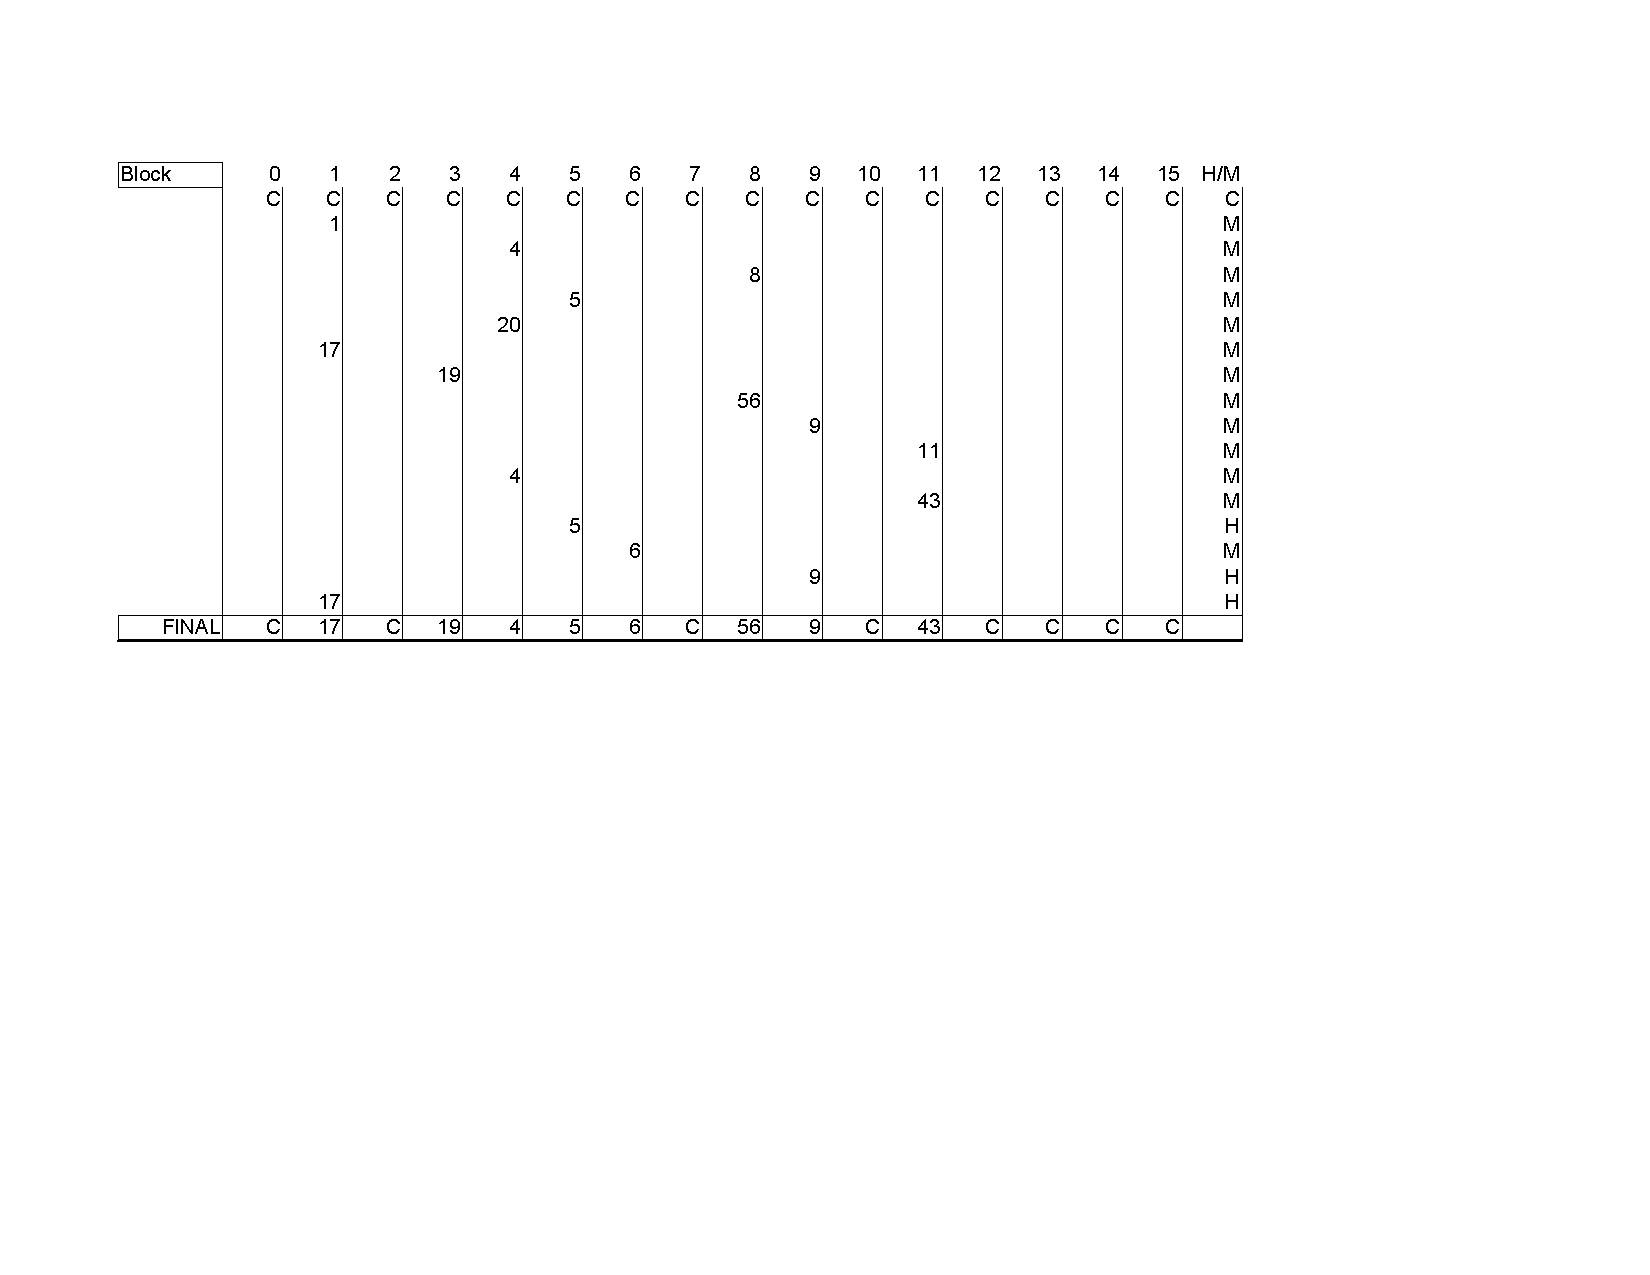
\includegraphics[trim = 0in 3.5in 0inin 1in, scale=0.6]{1a.pdf}
\end{center}

The following diagram shows the C2 cache. The reads are boxed, and the cached items  are all written on the same line. Hits and misses are on the right. On the bottom you see the final state of the cache.
\begin{center}
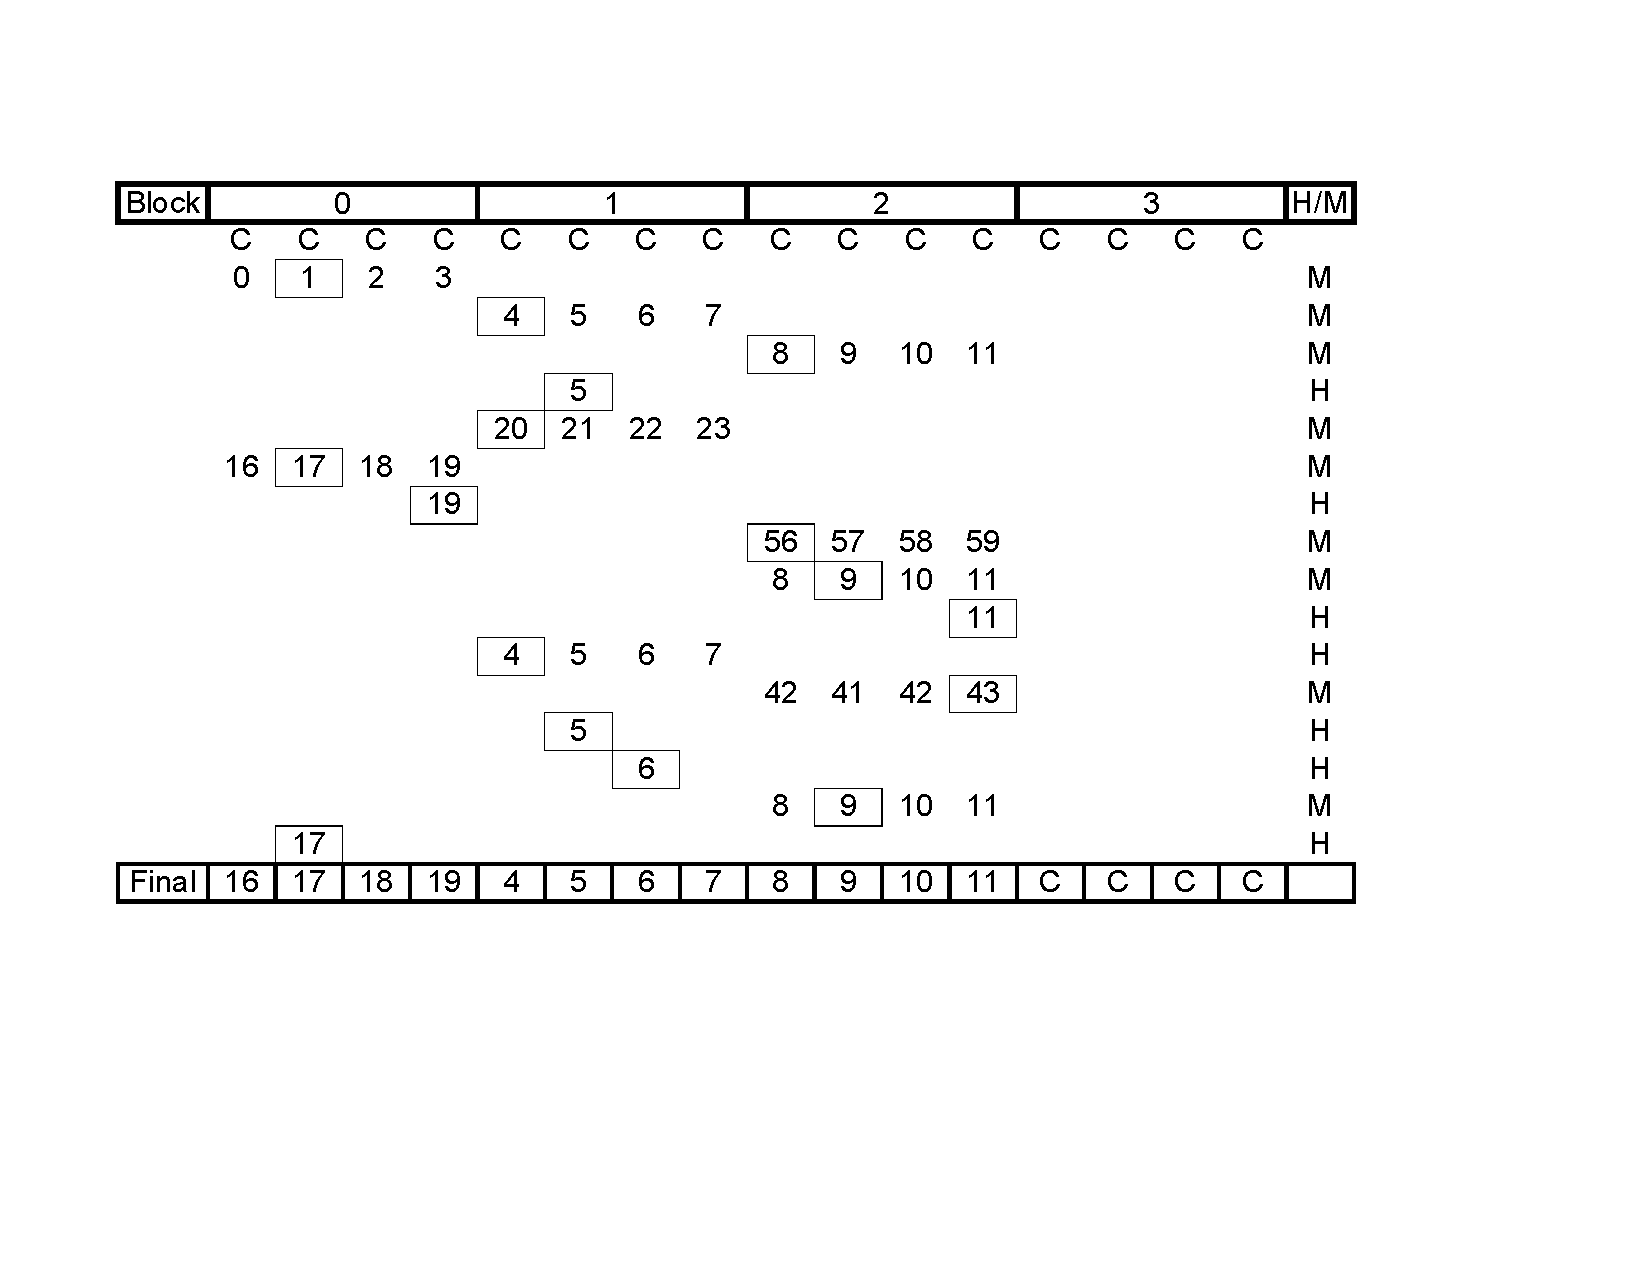
\includegraphics[trim=0 2.5in 0 1in,scale=0.5]{1b.pdf}
\end{center}

b.) Addresses read: 0, 1, 4, 8.\\
C1 has 4 misses. 4(8) = 32.\\
C2 has 3 misses 3(11) = 33.\\

c.)  Addresses read: 0, 3, 16, 3, 16.\\
C1: M M M H H\\
C2: M H M M M\\

\textbf{Problem 2}\\
a.)$ C = A \times B \times S$ \\
$S = \frac{C}{A\times B}$\\

b.)The total number of bits needed is  the number of sets times the number of lines per set times the number of bits per line. So,  we need $S\times A \times (1 + t + B*8)$.\\
Where the 1 accounts for the valid bit, t acounts for the tag bits per line and B*8 accounts for the block size in bits.\\
$S = 2^s$, $B = 2^b$, and $t = k - (b + s)$.\\
So, $t = k - (log_2(S) + log_2(B))$. Also, $A\times S = \frac{C}{2^b}.$\\
The answer is $\frac C{2^b}\times (1+ k - log_2(\frac{C}{A\times B}) - b + 2^b*8)$\\
(There is no dirty bit in this exercise.)\\

\textbf{Problem 3} One of three things could happen. We could hit the L1 cache, we could  miss the L1 cache, but hit the L2 cache, or we could miss both. Let $m_1$  be the miss rate for L1, and let $m_2$ be the miss rate for L2. Then, according to \cite{L2}:

\begin{equation}
AMAT = t_h^1 + m_1\times(t_h^2+m_2\times t_m^2)
\end{equation}
a.)	$size \le C1$. Then the miss rate for L1 is once per cache line, or $\frac{1}{B1}$, on the first iteration, and never during the subsequent iterations, since after the first iteration all of A will be stored in the cache. L2 will have half the miss rate of L1 since it has a twice bigger line size. Again, there will be no miss on the subsequent iterations since all of A will already be cached. So, we will add 99 L1 hit times to the access time, and then divide by 100.
\begin{equation}
AMAT = \frac1{100}[(t_h^1+\frac{1}{B1}(t_h^2 + \frac{1}{2*B1}*t_m^2)) + 99*t_h^1]
\end{equation}

b.) $C1 < size \le C2.$ Now all of A will not fit in C1, and some lines in C1 may be overwritten as we sum through A. 
In fact, we need to consider two cases. \\
i.) $C1< size \le 2C1$
In this case, part of the C1 cache will need to be loaded once, and another part will be loaded during each iteration of it.  During the first iteration, the miss rate will be $\frac{1}{B1}$. Later, the miss rate will be $\frac{1}{B1}$ for some only some blocks, while it is possible if size < 2C1 that some blocks wont be updated. For convenience of notation, let's let $S_A =ceil(size/B1)$ be the number of sets needed to contain array A, and lets let $S1 = C1/B1$ be the number of sets in C1. The fraction of sets of data which will have a miss per block is $\frac{S_A - S1mod(S_A - S1)}{S_A}$. We will have a miss rate of $\frac1{2*diB1}$ for C2 during the first iteration of it, but during subsequent iterations of it all of A will be in C2 and we will have no misses. See the image on the next page for more explanantion.
\begin{equation}
AMAT = \frac{1}{100}[(t_h^1+\frac{1}{B1}(t_h^2 + \frac{1}{2*B1}*t_m^2) + 99*(t_h^1+(\frac{S_A - S1mod(S_A - S1)}{S_A})\frac{1}{B1}(t_h^2))]
\end{equation}

Note that if $S_A$ is a multiple of $S1$, that is $S_A = n*S1$, $S1mod(S_A-S1) = S1mod((n-1)S1) = 0$, and the C1 cache is completely overwritten each time we loop it, and the miss rate for $C1$ is $\frac1{B1}$, or, once per block.

ii.) $2C1 < size \le C2$. In this case, all of C1 will need to be wiped clean during each iteration of it. C2 will need to be filled only during the first loop  or it.
\begin{equation}
AMAT = \frac1{100}[(t_h^1+\frac{1}{B1}(t_h^2 + \frac{1}{2*B1}*t_m^2)) + 99*(t_h^1 + \frac{1}{B1}(t_h^2))]
\end{equation}


C.) $size > C2$.
This case also needs to be broken down into subcases. Either the whole C2 cache is overwritten during each loop of it, or only a portion of it changes.\\ 
i.) $C2 < size \le 2*C2$.
In this case, we need to determine which parts of C2 are not overwritten during the loop. Of course, during the first iteration all of C2 must be filled. Let $S_A = ceil(size/(2*B1))$ and let $S_2 = C2/(2*B1)$. Then, similar to 2i., we get:
\begin{equation}
AMAT = \frac1{100}[t_h^1 + \frac{1}{B1}*(t_h^2+\frac{1}{2*B1}* t_m^2)+99*(t_h^1 + \frac{1}{B1}*(t_h^2+\frac{S_A - S2mod(S_A - S2)}{S_A}\frac{1}{2*B1}* t_m^2))]
\end{equation}

ii.) $2*C2 < size$.
In this case the whole C1 and C2 caches are completely overwritten multiple times during each iteration of it.
\begin{equation}
AMAT = t_h^1 + \frac{1}{B1}*(t_h^2+\frac{1}{2*B1}* t_m^2)
\end{equation}
\newpage
\begin{center}
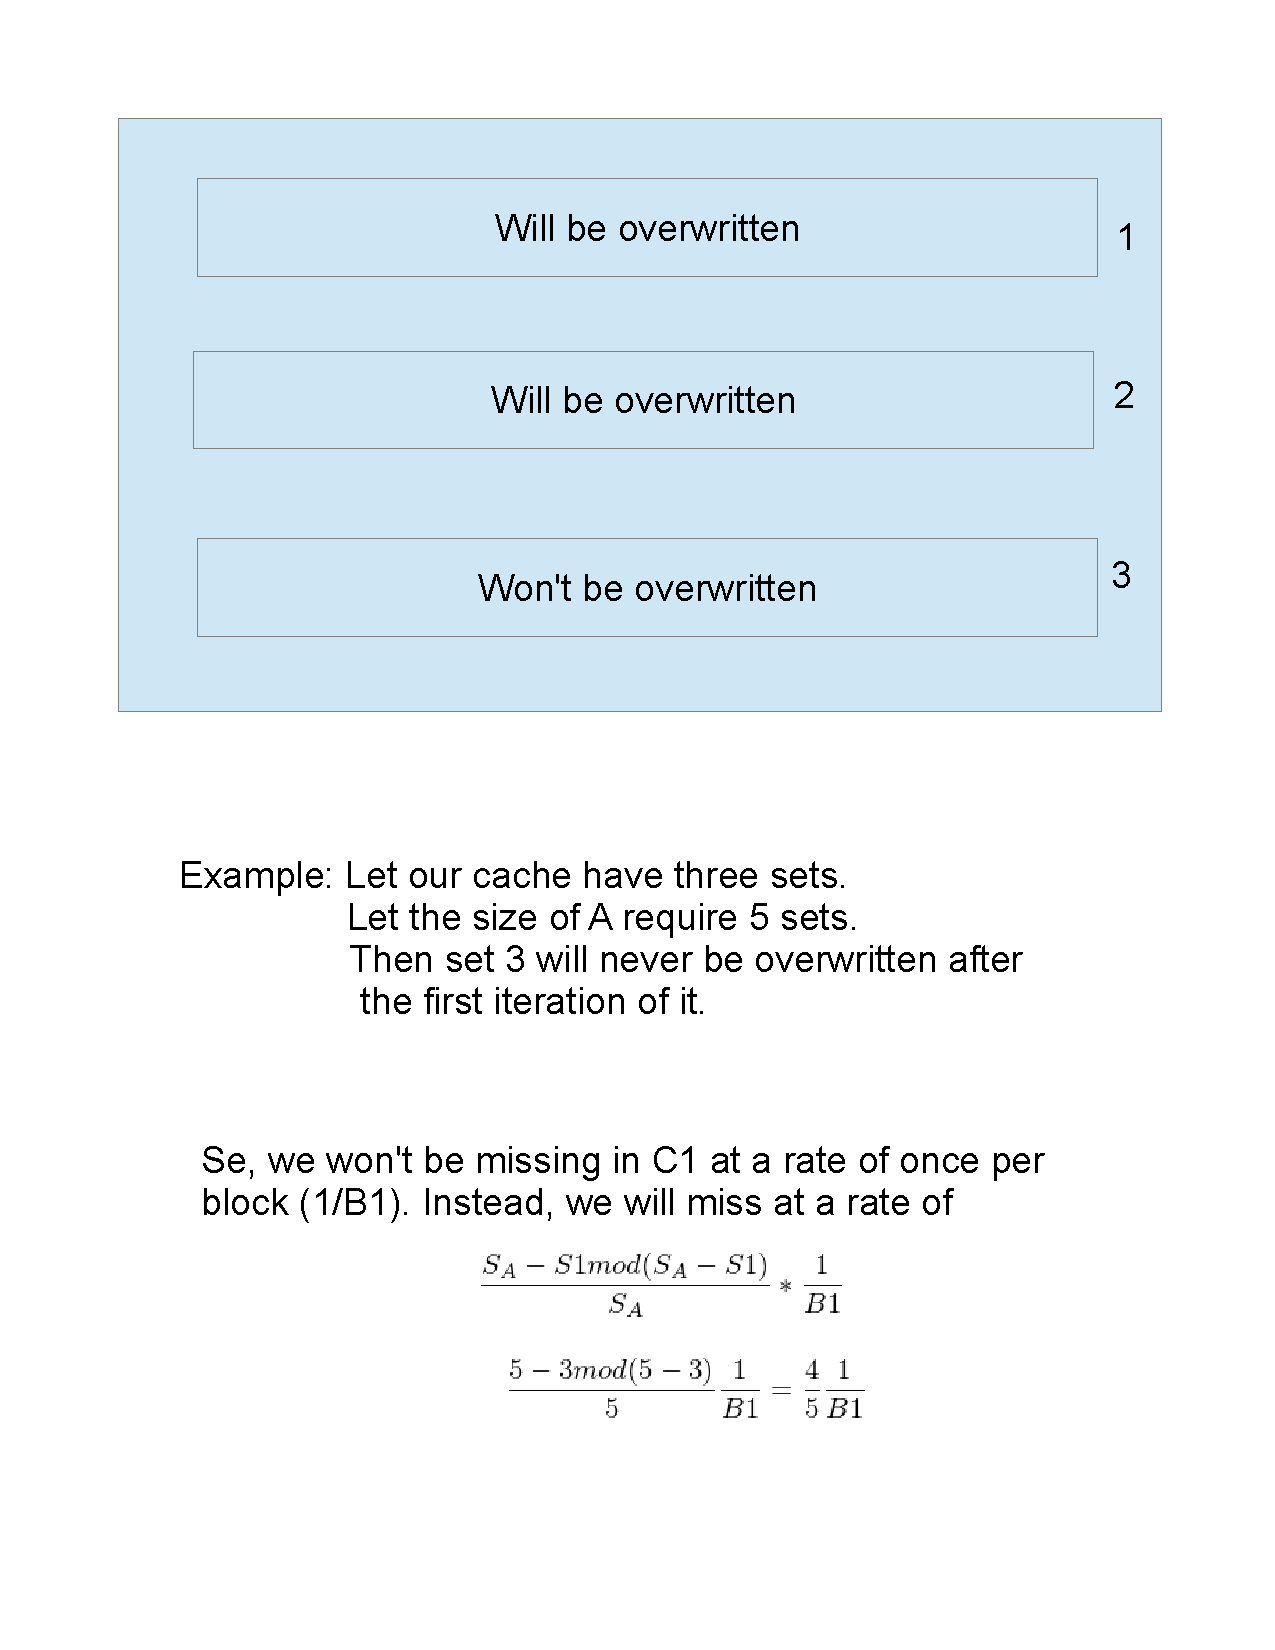
\includegraphics[scale = 0.6]{L2.pdf}
\end{center}
\begin{thebibliography}{9}
\bibitem{Avi}
  Avi,
  \emph{Finding cache block transfer time in a 3 level memory system}.
cs.stackexchange.com. 14 April 2013.http://cs.stackexchange.com/questions/29738/l1-and-l2-cache
\bibitem{Melvyn} Cienfuegos, Julian, cs.stackexchange.com/questions/29738/l1-and-l2-cache. 8 September 2014.
\bibitem{How}\emph{How Caching Works}, http://computer.howstuffworks.com/cache4.htm, 8 September 2014.
\bibitem{L2} Computer Architecture: AMAT. http://www.nu.edu.sa/userfiles/sralmasud/Computer\%20Architecture13.pdf. 8 Sept 2014
\end{thebibliography}
\end{document}


